\subsection{RAID 6}

RAID 6 es una extensión de RAID 5 que incorpora doble paridad distribuida. Su principal objetivo es aumentar la tolerancia a fallos, permitiendo que el arreglo continúe funcionando incluso si fallan simultáneamente dos discos.

Al igual que RAID 5, los datos se distribuyen mediante striping a nivel de bloques, pero cada conjunto de datos genera dos bloques de paridad independientes, que también se distribuyen entre todos los discos.

Un ejemplo conceptual con cuatro discos se muestra en la figura \ref{fig:raid6}.

\begin{figure}[!ht]
  \centering
  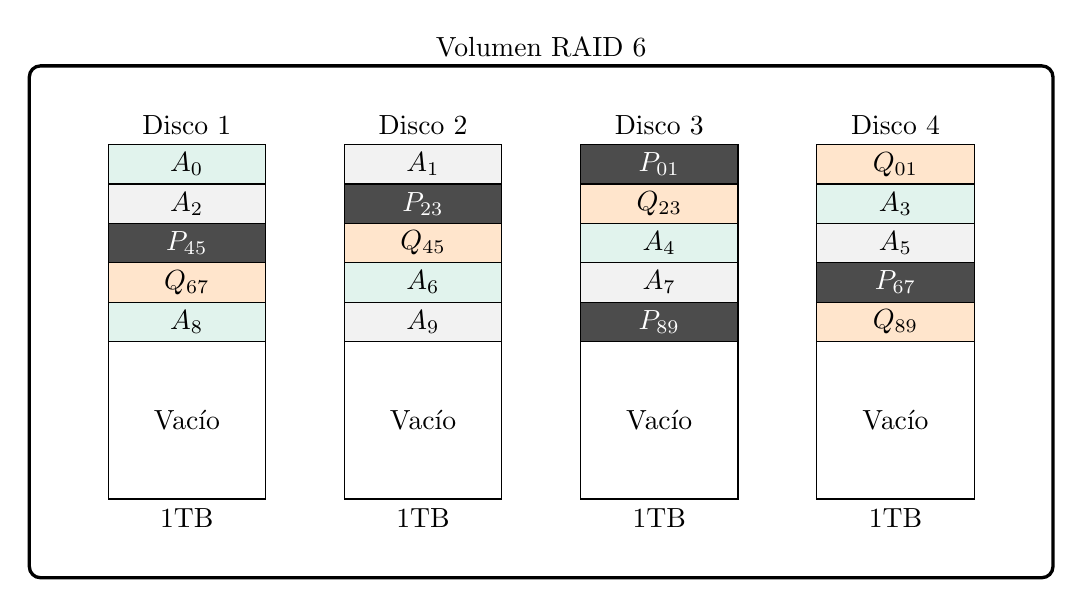
\begin{tikzpicture}
    \node[above] at (1,2.5) {Disco 1};
    \foreach \y\t\c in {
        0/A_8/white!95!blue!93!green,
        0.5/Q_{67}/orange!20,
        1/\color{white}P_{45}/black!70,
        1.5/A_2/gray!10,
        2/A_0/white!95!blue!93!green}{
      \draw[fill=\c] (0,\y) rectangle node{\(\t\)} (2,{0.5+\y});
    }
    \draw (0,0) rectangle node{Vacío} (2,-2);
    \node[below] at (1,-2) {1TB};

    \node[above] at (4,2.5) {Disco 2};
    \foreach \y\t\c in {
        0/A_9/gray!10,
        0.5/A_6/white!95!blue!93!green,
        1/Q_{45}/orange!20,
        1.5/\color{white}P_{23}/black!70,
        2/A_1/gray!10}{
      \draw[fill=\c] (3,\y) rectangle node{\(\t\)} (5,{0.5+\y});
    }
    \draw (3,0) rectangle node{Vacío} (5,-2);
    \node[below] at (4,-2) {1TB};

    \node[above] at (7,2.5) {Disco 3};
    \foreach \y\t\c in {
        0/\color{white}P_{89}/black!70,
        0.5/A_7/gray!10,
        1/A_4/white!95!blue!93!green,
        1.5/Q_{23}/orange!20,
        2/\color{white}P_{01}/black!70}{
      \draw[fill=\c] (6,\y) rectangle node{\(\t\)} (8,{0.5+\y});
    }
    \draw (6,0) rectangle node{Vacío} (8,-2);
    \node[below] at (7,-2) {1TB};

    \node[above] at (10,2.5) {Disco 4};
    \foreach \y\t\c in {
        0/Q_{89}/orange!20,
        0.5/\color{white}P_{67}/black!70,
        1/A_5/gray!10,
        1.5/A_3/white!95!blue!93!green,
        2/Q_{01}/orange!20}{
      \draw[fill=\c] (9,\y) rectangle node{\(\t\)} (11,{0.5+\y});
    }
    \draw (9,0) rectangle node{Vacío} (11,-2);
    \node[below] at (10,-2) {1TB};

    \draw[very thick,rounded corners] (-1,-3) rectangle (12,3.5);
    \node[above] at (5.5,3.5) {Volumen RAID 6};
  \end{tikzpicture}
  \caption{Tamaño del volumen de RAID 6: 2TB.}
  \label{fig:raid6}
\end{figure}

Donde:
\begin{itemize}
  \item P representa la primera paridad.
  \item Q representa la segunda paridad.
  \item Ambas se distribuyen entre todos los discos.
\end{itemize}
A diferencia de RAID 5, donde la paridad suele calcularse mediante una operación XOR, RAID 6 utiliza dos algoritmos de paridad distintos (uno de ellos suele ser XOR y el otro se basa en códigos de corrección, como Reed--Solomon). Gracias a ello, es posible recuperar la información incluso cuando se pierden los datos de dos discos.

\paragraph{Ventajas:}
\begin{itemize}
  \item Tolera la falla simultánea de dos discos.
  \item Muy alta disponibilidad y seguridad de los datos.
  \item La paridad está distribuida, por lo que no existe un disco dedicado que limite el rendimiento.
\end{itemize}

\paragraph{Desventajas:}
\begin{itemize}
  \item Las escrituras son más lentas que en RAID 5, ya que deben calcularse y actualizarse dos paridades.
  \item Requiere al menos cuatro discos.
  \item La implementación es más compleja.
\end{itemize}

\paragraph{Velocidad de Escritura}
Al igual que con RAID 5, depende de la controladora RAID, ya que requiere calcular dos paridades entre los datos del Disco de datos 1 y el Disco de datos 2. A modo de ejemplo si se tiene \(A_0\) y se inserta \(A_1\), una escritura tendrá las siguientes cuatro operaciones:
\begin{enumerate}
  \item Escribir \(A_1\)
  \item Leer \(A_0\)
  \item Calcular \(P_{01}\)
  \item Escribir \(P_{01}\)
  \item Calcular \(Q_{01}\)
  \item Escribir \(Q_{01}\)
\end{enumerate}

De este modo, si se supone la velocidad del Disco igual a 100~MB/s, resulta que 
\[
  \text{Velocidad de escritura relativa a un disco} = \frac{100~\text{MB/s}}{6} = 16.6~\text{MB/s}
\]

\begin{table}[!ht]
  \centering
  \begin{tabular}{l|c}
    Cantidad de discos mínima & 4 \\\hline
    Cantidad de discos que pueden fallar & 2 \\ \hline
    Velocidad de escritura relativa a un disco & \(\frac{\text{VDisco}}{\text{Cant. Oper.}}\)~[MB/s] \\\hline
    Velocidad de escritura ponderada & 2 \\ \hline
    Velocidad de lectura relativa a un disco & VDisco~[MB/s] \\ \hline
    Velocidad de lectura ponderada & 5 \\ \hline
    Costo & Alto
  \end{tabular}
  \caption{Características del RAID 6.}
\end{table}

\paragraph{Ejemplo}
Con seis discos de 1 TB:
\begin{itemize}
  \item Capacidad física total: 6 TB.
  \item Capacidad útil: 4 TB (la capacidad equivalente a dos discos se utiliza para la doble paridad).
  \item El sistema puede soportar la falla de dos discos sin perder información.
\end{itemize}
